\section{Matrix Element Analysis Technique} 

\subsection{Introduction}
\label{me_intro}
The matrix element analysis uses leading order matrix elements to separate single top quark events from W+jets and $\ttbar$ background events. The matrix element analysis calculates a probability for an event to be a signal top event, either s-channel or t-channel, and a probability for one of several W+jets backgrounds. This probability is defined in equation ~\ref{prob}.

\begin{equation}
\label{prob}
P(\vec{x}) = \frac{1}{\sigma} \sum_{i,j} \int f_{i}(x_{1}, Q^{2})dx_{1}
\times 
f_{j}(x_{2}, Q^{2})dx_{2} \times \pderiv{\sigma_{hs,ij}(\vec{y})}{\vec{y}} \times W(\vec{x},\vec{y})d\vec{y}
\end{equation}

where $f(x_{i},Q^{2})$ is the parton distribution function for parton i,  $\pderiv{\sigma_{hs,ij}(\vec{y})}{\vec{y}}$ is the differential cross section for the hard scatter interaction, and $W(\vec{x},\vec{y})$ is the probability that final state $\vec{y}$ is reconstructed as $\vec{x}$ in the detector, and finally, $\sigma$ is an overall normalization constant defined as the integral of the differential cross section over the entire detector phase space, $d\vec{x}$ as shown in equation ~\ref{prob2}.
\begin{equation}
\label{prob2}
\sigma = \sum_{i,j} \int f_{i}(x_{1}, Q^{2})dx_{1}
\times 
f_{j}(x_{2}, Q^{2})dx_{2} \times \pderiv{\sigma_{hs,ij}(\vec{y})}{\vec{y}} \times W(\vec{x},\vec{y})d\vec{y}d\vec{x}
\end{equation}

This analysis uses CTEQ 6.1 LO parton distribution functions accessed via
LHAPDF C++ wrapper~\footnote{http://hepforge.cedar.ac.uk/lhapdf/}. The matrix elements are calculated using the MadGraph leading order
matrix element generator.

\subsection{Jet-Parton Assignment}
The event probabilities calculated in section ~\ref{me_intro} assume a particle assignment of a jet to a parton in the final state. In practice, this assignment is not known and we must sum over all possible assignments to ensure the correct one is chosen.
For two jet events, the event probability is then re-written as a sum over assignment possibilities as shown in equation ~\ref{assign}

\begin{eqnarray}
\label{assign}
\nonumber
P(\ell, \nu, \vec{\rm{jets}}) = \alpha_{1 \rightarrow 1;2 \rightarrow 2} \times P(\ell, \nu, \rm{j}_{1} \rightarrow p_{1}, j_{2} \rightarrow p_{2}) + \\
\alpha_{1 \rightarrow 2; 2 \rightarrow 1} \times P(\ell, \nu, \rm{j}_{1} \rightarrow p_{2}, j_{2} \rightarrow p_{1})
\end{eqnarray}

where the coefficients, $\alpha$, are free parameters that depend on the jet-parton assignment probability. Determination of these parameters is described in appendix ~\ref{jpassign}. For three jet events, the event probability is defined as

\begin{eqnarray}
\label{assign}
\nonumber
P(\ell, \nu, \vec{\rm{jets}}) = 
\alpha_{1 \rightarrow 1;2 \rightarrow 2; 3 \rightarrow 3} \times P(\ell, \nu, \rm{j}_{1} \rightarrow p_{1}, j_{2} \rightarrow p_{2}, j_{3} \rightarrow p_{3}) + \\
\nonumber
\alpha_{1 \rightarrow 1;2 \rightarrow 3; 3 \rightarrow 2} \times P(\ell, \nu, \rm{j}_{1} \rightarrow p_{1}, j_{2} \rightarrow p_{3}, j_{3} \rightarrow p_{2}) + \\
\nonumber
\alpha_{1 \rightarrow 2;2 \rightarrow 1; 3 \rightarrow 3} \times P(\ell, \nu, \rm{j}_{1} \rightarrow p_{2}, j_{2} \rightarrow p_{1}, j_{3} \rightarrow p_{3}) + \\
\nonumber
\alpha_{1 \rightarrow 2;2 \rightarrow 3; 3 \rightarrow 1} \times P(\ell, \nu, \rm{j}_{1} \rightarrow p_{2}, j_{2} \rightarrow p_{3}, j_{3} \rightarrow p_{1}) + \\
\nonumber
\alpha_{1 \rightarrow 3;2 \rightarrow 2; 3 \rightarrow 1} \times P(\ell, \nu, \rm{j}_{1} \rightarrow p_{3}, j_{2} \rightarrow p_{2}, j_{3} \rightarrow p_{1}) + \\
\alpha_{1 \rightarrow 3;2 \rightarrow 1; 3 \rightarrow 2} \times P(\ell, \nu, \rm{j}_{1} \rightarrow p_{3}, j_{2} \rightarrow p_{1}, j_{3} \rightarrow p_{2})
\end{eqnarray}

\subsection{Matrix Element Analysis Output}
The matrix element analysis is named so because the differential cross section for the hard scatter interaction is proportional to the leading order matrix element as shown in equation ~\ref{me}

\begin{equation}
\label{me}
d\sigma_{hs} = \frac{(2\pi)^4}{4} \frac{{|\cal M|}^{2}}{\sqrt{(q_{1}q_{2})^2 - m_{1}^2
m_{2}^2}} d\Phi_{n}(y)
\end{equation}

For this analysis, we consider four probabilities for two jet events and and three probabilities for three jet events. For two jet events events, we calculate the probability for s-channel single top ($u\bar{d}$ $\rightarrow$ $t\bar{b}$), t-channel single top ($ub$ $\rightarrow$ $td$), Wbb production ($u\bar{d}$ $\rightarrow$ $Wb\bar{b}$), and Wcg production ($sg$ $\rightarrow$ $W\bar{c}g$). The leading order diagrams for these channels are shown in figure ~\ref{2jets}.

\vspace{0.1in}
\begin{figure}[!h!tbp]
\begin{center}
\subfigure[]{
	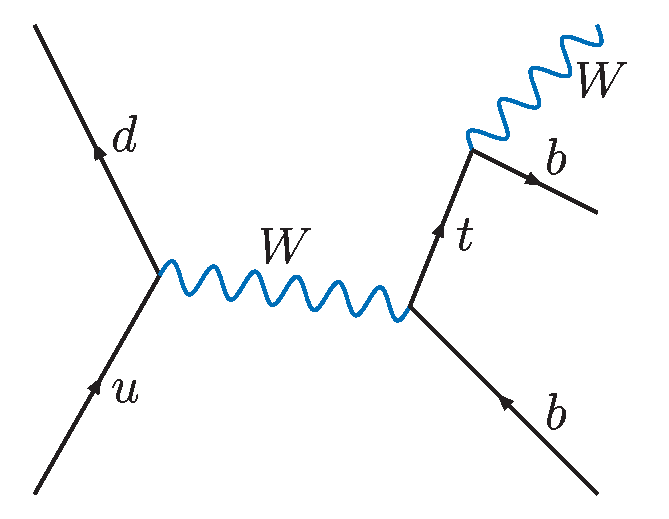
\includegraphics[width=0.22\textwidth]{figures/tb.eps}
}
\subfigure[]{
	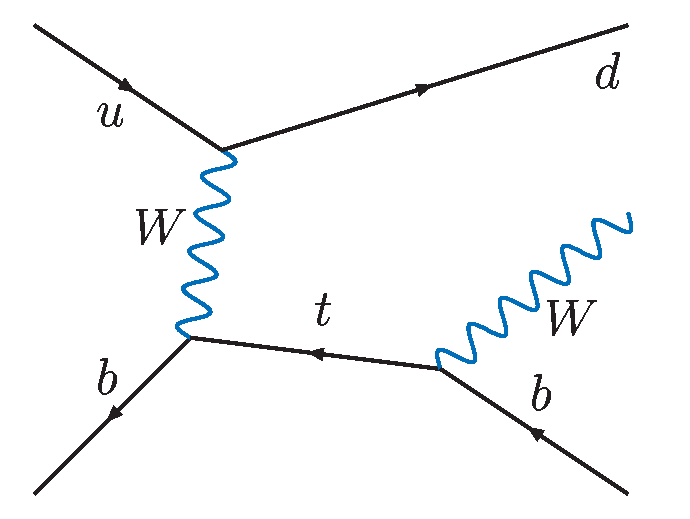
\includegraphics[width=0.22\textwidth]{figures/tq.eps}
}
\subfigure[]{
	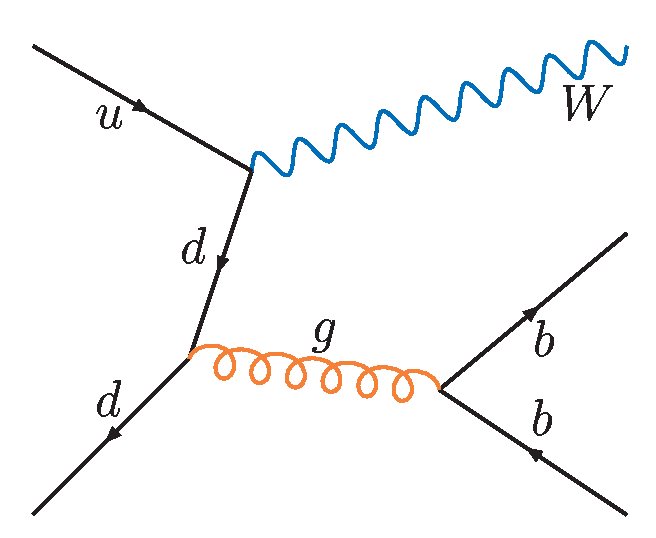
\includegraphics[width=0.22\textwidth]{figures/wbb.eps}
}
\subfigure[]{
	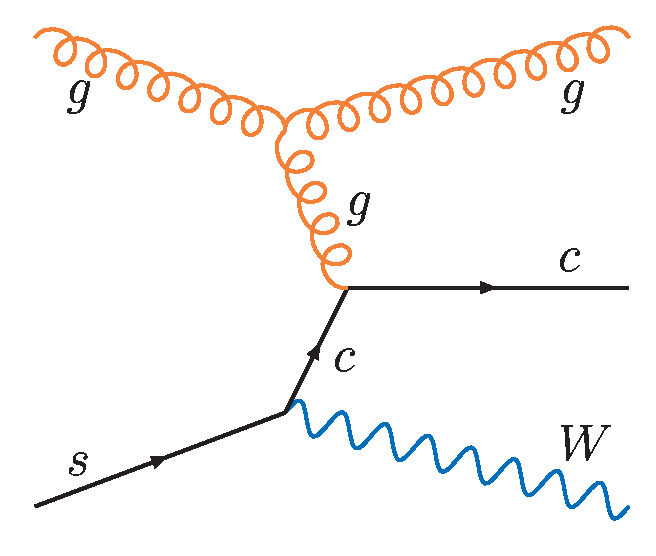
\includegraphics[width=0.22\textwidth]{figures/wcg.eps}
}
\end{center}
\vspace{-0.1in}
\caption[2jets]{The leading order matrix elements used for event probability calculation for events with two jets. (a) $u\bar{d}$ $\rightarrow$ $t\bar{b}$, (b) $ub$ $\rightarrow$ $td$, (c) $u\bar{d}$ $\rightarrow$ $Wb\bar{b}$, (d) $sg$ $\rightarrow$ $W\bar{c}g$}
\label{2jets}
\end{figure}

For events with three jets, we use three matrix elements, s-channel with gluon radiation ($u\bar{d}$ $\rightarrow$ $t\bar{b}g$), t-channel with associated b quark ($ug$ $\rightarrow$ $t\bar{b}d$), and Wbbg ($u\bar{d}$ $\rightarrow$ $Wb\bar{b}g$). The leading order Feynman diagrams are shown in figure ~\ref{3jets}.

\vspace{0.1in}
\begin{figure}[!h!tbp]
\begin{center}
\subfigure[]{
	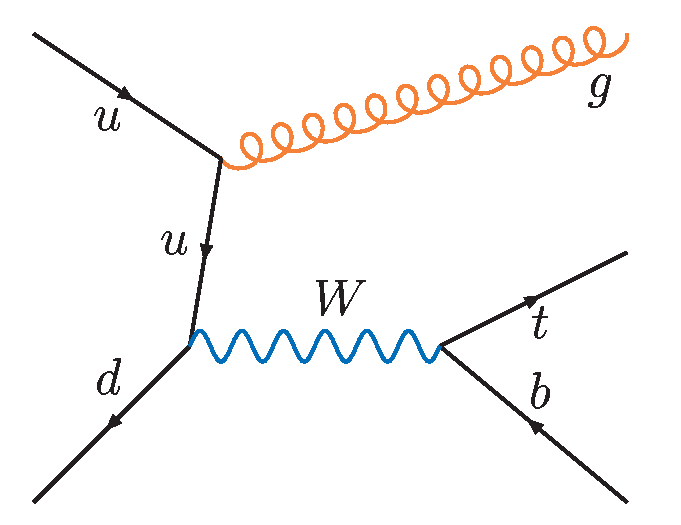
\includegraphics[width=0.22\textwidth]{figures/tbg.eps}
}
\subfigure[]{
	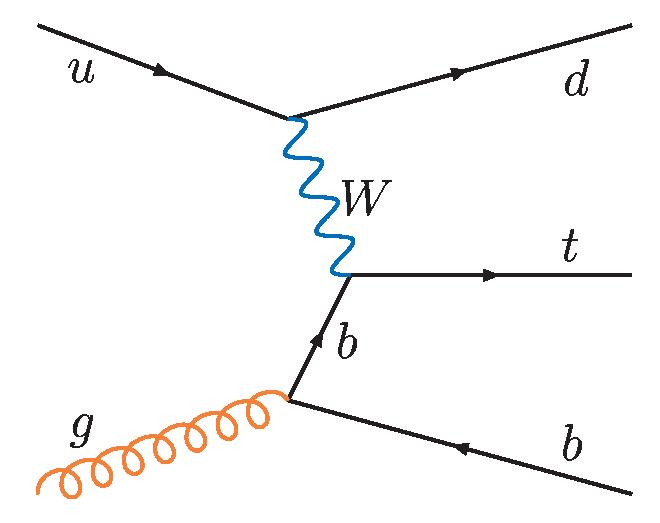
\includegraphics[width=0.22\textwidth]{figures/tqb.eps}
}
\subfigure[]{
	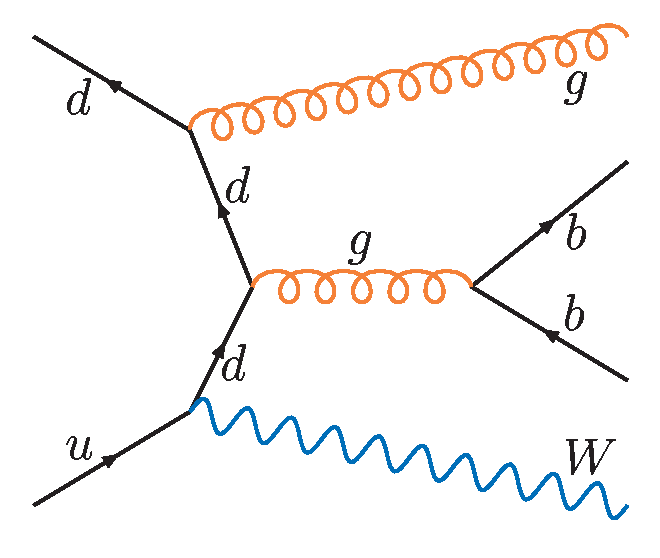
\includegraphics[width=0.22\textwidth]{figures/wbbg.eps}
}
\end{center}
\vspace{-0.1in}
\caption[3jets]{The leading order matrix elements used for event probability calculation for events with two jets.  (a) $u\bar{d}$ $\rightarrow$ $t\bar{b}g$, (b) $ug$ $\rightarrow$ $t\bar{b}d$, (c) $u\bar{d}$ $\rightarrow$ $Wb\bar{b}g$}
\label{3jets}
\end{figure}

After calculating event probabilities we combine them into a discriminant output variable, D, defined in equation ~\ref{disc}

\begin{equation}
\label{disc}
D(\vec{x}) = \frac{P_{\rm{signal}}(\vec{x})}{P_{\rm{signal}}(\vec{x}) + P_{\rm{background}}(\vec{x})}
\end{equation}

where $c_{wbb}$ and $c_{wcg}$ are, in principle, the relative background fractions for each background in the data; however, these background fractions are optimizable for the analysis. 

For events with two jets the discriminant for either s-channel or t-channel as signal is defined as

\begin{equation}
D(\vec{x})_{\rm{s|t}} = \frac{P_{\rm{s|t}}(\vec{x})}{P_{\rm{st}}(\vec{x}) + c_{wbb}P_{\rm{wbb}}(\vec{x}) + c_{wcg}P_{\rm{wcg}}(\vec{x})}
\end{equation}

and events with three jets the discriminant for s-channel and t-channel is defined as

\begin{equation}
D(\vec{x})_{\rm{s|t}} = \frac{P_{\rm{s|t}}(\vec{x})}{P_{\rm{st}}(\vec{x}) + P_{\rm{wbbg}}(\vec{x})}
\end{equation}




